\documentclass{report}

\usepackage[utf8]{inputenc}
\usepackage{url}
\usepackage{mdframed}
\usepackage{graphicx}
\usepackage{xspace}
\usepackage{amsmath}
\usepackage{listings} % For code formatting

% Configuration for code listings
\lstset{
    basicstyle=\ttfamily\small,
    frame=single,
    numbers=left,
    numberstyle=\tiny,
    keywordstyle=\color{blue}\bfseries,
    commentstyle=\color{gray},
    stringstyle=\color{red},
    showstringspaces=false,
    breaklines=true,
    postbreak=\mbox{\textcolor{red}{$\hookrightarrow$}\space},
    tabsize=2
}

\begin{document}

\begin{titlepage}
\centering
\vspace*{\fill}
\huge{\textbf{CS3008: IMAGE AND VIDEO PROCESSING}}\\
\vspace{1 cm}

\begin{mdframed}
\centering
\LARGE{\textbf{LABORATORY REPORTS}}
\end{mdframed}

\vspace{3 cm}

\begin{flushleft}
\large{\textbf{Name: Jayashre\\
Roll No.: 22011103020 \\
College: Shiv Nadar University, Chennai\\}}

\vspace*{\fill}

\end{flushleft}
\end{titlepage}

\chapter{Eye Detection Using OpenCV} % Enable numbering for chapter

\section{Abstract}
This report documents the implementation of an eye detection system using the OpenCV library. The system utilizes Haar cascade classifiers to identify faces and eyes in images and marks them with bounding boxes. The project aims to provide a foundational understanding of image processing techniques and their practical applications.

\section{Introduction}
Eye detection plays a vital role in computer vision applications such as gaze tracking, facial recognition, and user interaction systems. This project implements a detection system using pre-trained Haar cascade classifiers, which efficiently identify facial and ocular features in images.

\section{Methodology}
\subsection{Data Collection}
The input data consists of static images containing human faces. The images were uploaded manually in the Google Colab environment for processing.

\subsection{Tools and Libraries}
\begin{itemize}
    \item \textbf{OpenCV}: For image processing and detection.
    \item \textbf{Google Colab}: For executing Python code and visualizing results.
\end{itemize}

\subsection{Detection Algorithm}
The steps followed in the implementation are:
\begin{enumerate}
    \item Convert the input image to grayscale for easier processing.
    \item Use the Haar cascade classifier to detect faces in the image.
    \item For each detected face, apply the Haar cascade classifier for eyes within the facial region.
    \item Highlight the detected features (faces and eyes) using bounding boxes.
\end{enumerate}

\section{Implementation}
The implementation was carried out in Python using OpenCV. The following code snippet demonstrates the detection process:

\begin{lstlisting}[language=Python, caption=Eye Detection Code, label=code:eye-detection]
import cv2
face_cascade = cv2.CascadeClassifier(cv2.data.haarcascades + 'haarcascade_frontalface_default.xml')
eye_cascade = cv2.CascadeClassifier(cv2.data.haarcascades + 'haarcascade_eye.xml')
image = cv2.imread('input_image.jpg')
gray_image = cv2.cvtColor(image, cv2.COLOR_BGR2GRAY)
faces = face_cascade.detectMultiScale(gray_image, scaleFactor=1.1, minNeighbors=5)

for (x, y, w, h) in faces:
    cv2.rectangle(image, (x, y), (x+w, y+h), (255, 0, 0), 2)
    roi_gray = gray_image[y:y+h, x:x+w]
    roi_color = image[y:y+h, x:x+w]
    eyes = eye_cascade.detectMultiScale(roi_gray)
    for (ex, ey, ew, eh) in eyes:
        cv2.rectangle(roi_color, (ex, ey), (ex+ew, ey+eh), (0, 255, 0), 2)
cv2.imwrite('output_image.jpg', image)
cv2.imshow('Eye Detection', image)
cv2.waitKey(0)
cv2.destroyAllWindows()
\end{lstlisting}

\section{Results and Discussion}
The system was tested with several images under various conditions. The results are summarized below:
\begin{itemize}
    \item Faces were detected accurately in well-lit images.
    \item Eye detection was successful but occasionally struggled with images where faces were partially obscured.
\end{itemize}

\begin{figure}[h!]
    \centering
    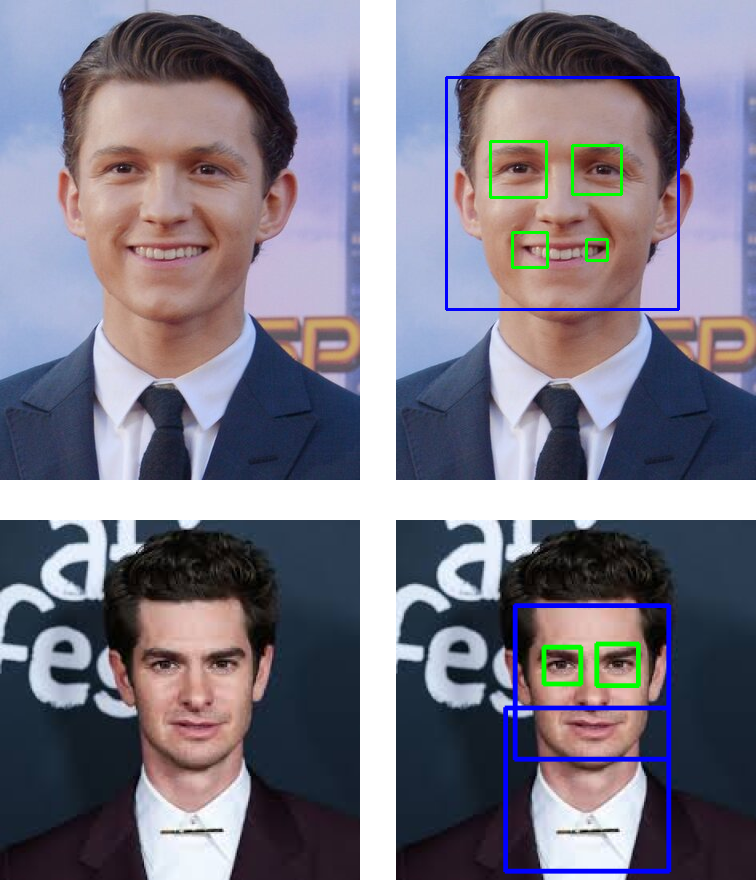
\includegraphics[width=0.4\textwidth]{images/Exp-1-Results.png} % Adjusted image size
    \caption{Detected faces and eyes in the input image.}
    \label{fig:output}
\end{figure}

\section{Conclusion}
The project successfully implemented an eye detection system using Haar cascades in OpenCV. While the system is efficient for basic detection, future improvements can involve the use of deep learning-based models for enhanced accuracy and robustness.

\end{document}
